\documentclass[UTF8,12pt]{ctexart}
\usepackage[a4paper,margin=24mm]{geometry}
\usepackage{amsmath,amssymb,bm,graphicx,adjustbox}
\newcommand{\fitmath}[1]{\begin{adjustbox}{max width=\linewidth}$\displaystyle #1$\end{adjustbox}}
\setlength{\parindent}{0pt}
\setlength{\parskip}{.7em}
\sloppy
\allowdisplaybreaks
\begin{document}
\section*{2016 年考研数学三 · 真题}
\subsection*{原 PDF 第 16 页}

\subsection*{2016年全国硕士研究生招生考试试题}

\subsection*{一、选择题（本题共8小题，每小题4分，共32分。在每小题给出的四个选项中，只有一项符合题目要求，把所选项前的字母填在题后的括号内。）}

（1）设函数 \(\displaystyle f(x)\) 在 \(\displaystyle (-\infty,\allowbreak +\infty)\) 内连续，其导函数的图形如图所示，则（　）。


\begin{center}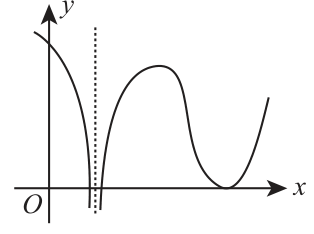
\includegraphics[width=.85\linewidth]{../assets/figures/page-016-03.png}\end{center}

（A）函数 \(\displaystyle f(x)\) 有2个极值点，曲线 \(\displaystyle y=f(x)\) 有2个拐点。 （B）函数 \(\displaystyle f(x)\) 有2个极值点，曲线 \(\displaystyle y=f(x)\) 有3个拐点。 （C）函数 \(\displaystyle f(x)\) 有3个极值点，曲线 \(\displaystyle y=f(x)\) 有1个拐点。 （D）函数 \(\displaystyle f(x)\) 有3个极值点，曲线 \(\displaystyle y=f(x)\) 有2个拐点。


（2）已知函数 \(\displaystyle f(x,\allowbreak y)=\dfrac{\displaystyle e^x}{\displaystyle x-y}\)，则（　）。


（A）\(\displaystyle f_x^{\prime}-f_y^{\prime}=0\)。 （B）\(\displaystyle f_x^{\prime}+f_y^{\prime}=0\)。 （C）\(\displaystyle f_x^{\prime}-f_y^{\prime}=f\)。 （D）\(\displaystyle f_x^{\prime}+f_y^{\prime}=f\)。


（3）设 \(\displaystyle J_i=\displaystyle \iint_{D_i}\sqrt[3]{x-y}\,\mathrm dx\mathrm dy\;(i=1,\allowbreak 2,\allowbreak 3)\)，其中 \(\displaystyle D_1=\{(x,\allowbreak y)\mid0\le x\le1,\allowbreak 0\le y\le1\}\)，\(\displaystyle D_2=\{(x,\allowbreak y)\mid0\le x\le1,\allowbreak 0\le y\le\sqrt x\}\)，\(\displaystyle D_3=\{(x,\allowbreak y)\mid0\le x\le1,\allowbreak x^2\le y\le1\}\)，则（　）。


（A）\(\displaystyle J_1<J_2<J_3\)。 （B）\(\displaystyle J_3<J_1<J_2\)。 （C）\(\displaystyle J_2<J_3<J_1\)。 （D）\(\displaystyle J_2<J_1<J_3\)。


（4）级数 \(\displaystyle \sum_{n=1}^{\infty}(\dfrac{\displaystyle 1}{\displaystyle \sqrt n}-\dfrac{\displaystyle 1}{\displaystyle \sqrt{n+1}})\sin(n+k)\)（\(\displaystyle k\) 为常数）（　）。


（A）绝对收敛。 （B）条件收敛。 （C）发散。 （D）收敛性与 \(\displaystyle k\) 有关。


（5）设 \(\displaystyle A,\allowbreak B\) 是可逆矩阵，且 \(\displaystyle A\) 与 \(\displaystyle B\) 相似，则下列结论错误的是（　）。


（A）\(\displaystyle A^{\mathrm T}\) 与 \(\displaystyle B^{\mathrm T}\) 相似。 （B）\(\displaystyle A^{-1}\) 与 \(\displaystyle B^{-1}\) 相似。 （C）\(\displaystyle A+A^{\mathrm T}\) 与 \(\displaystyle B+B^{\mathrm T}\) 相似。 （D）\(\displaystyle A+A^{-1}\) 与 \(\displaystyle B+B^{-1}\) 相似。


（6）设二次型 \(\displaystyle f(x_1,\allowbreak x_2,\allowbreak x_3)=a(x_1^2+x_2^2+x_3^2)+2x_1x_2+2x_2x_3+2x_1x_3\) 的正、负惯性指数分别为1，2，则（　）。


（A）\(\displaystyle a>1\)。 （B）\(\displaystyle a<-2\)。 （C）\(\displaystyle -2<a<1\)。 （D）\(\displaystyle a=1\) 或 \(\displaystyle a=-2\)。


（7）设 \(\displaystyle A,\allowbreak B\) 为两个随机事件，且 \(\displaystyle 0<P(A)<1\)，\(\displaystyle 0<P(B)<1\)，如果 \(\displaystyle P(A\mid B)=1\)，则（　）。


（A）\(\displaystyle P(\bar B\mid\bar A)=1\)。 （B）\(\displaystyle P(A\mid\bar B)=0\)。 （C）\(\displaystyle P(A\cup\bar B)=1\)。 （D）\(\displaystyle P(B\mid A)=1\)。


（8）设随机变量 \(\displaystyle X\) 与 \(\displaystyle Y\) 相互独立，且 \(\displaystyle X\sim N(1,\allowbreak 2)\)，\(\displaystyle Y\sim N(1,\allowbreak 4)\)，则 \(\displaystyle D(XY)=\)（　）。


（A）6。 （B）8。 （C）14。 （D）15。


\subsection*{二、填空题（本题共6小题，每小题4分，共24分，把答案填在题中横线上。）}

（9）已知函数 \(\displaystyle f(x)\) 满足 \(\displaystyle \lim_{x\to0}\dfrac{\displaystyle \sqrt{1+f(x)\sin2x}-1}{\displaystyle e^{3x}-1}=2\)，则 \(\displaystyle \lim_{x\to0}f(x)=\)\_\_\_\_\_\_。


\clearpage

\subsection*{原 PDF 第 17 页}

（10）极限 \(\displaystyle \lim_{n\to\infty}\dfrac{\displaystyle 1}{\displaystyle n^2}(\sin\dfrac{\displaystyle 1}{\displaystyle n}+2\sin\dfrac{\displaystyle 2}{\displaystyle n}+\cdots+n\sin\dfrac{\displaystyle n}{\displaystyle n})=\)\_\_\_\_\_\_。


（11）设函数 \(\displaystyle f(u,\allowbreak v)\) 可微，\(\displaystyle z=z(x,\allowbreak y)\) 由方程 \(\displaystyle (x+1)z-y^2=x^2f(x-z,\allowbreak y)\) 确定，则 \(\displaystyle \left.\mathrm dz\right|_{(0,\allowbreak 1)}=\)\_\_\_\_\_\_。


（12）设 \(\displaystyle D=\{(x,\allowbreak y)\mid|x|\le y\le1,\allowbreak -1\le x\le1\}\)，则 \(\displaystyle \iint_Dx^2e^{-y^2}\,\mathrm dx\mathrm dy=\)\_\_\_\_\_\_。


（13）行列式 \(\displaystyle \begin{vmatrix}\lambda&-1&0&0\\0&\lambda&-1&0\\0&0&\lambda&-1\\4&3&2&\lambda+1\end{vmatrix}=\)\_\_\_\_\_\_。


（14）设袋中有红、白、黑球各1个，从中有放回地取球，每次取1个，直到三种颜色的球都取到时停止，则取球次数恰好为4的概率为\_\_\_\_\_\_。


\subsection*{三、解答题（本题共9小题，共94分，解答应写出文字说明、证明过程或演算步骤。）}

（15）（本题满分10分）求极限 \(\displaystyle \lim_{x\to0}(\cos2x+2x\sin x)^{1/x^4}\)。


（16）（本题满分10分）设某商品的最大需求量为1200件，该商品的需求函数 \(\displaystyle Q=Q(p)\)，需求弹性 \(\displaystyle \eta=\dfrac{\displaystyle p}{\displaystyle 120-p}\;(\eta>0)\)，\(\displaystyle p\) 为单价（万元）。（I）求需求函数的表达式；（II）求 \(\displaystyle p=100\) 万元时的边际收益，并说明其经济意义。


\clearpage

\subsection*{原 PDF 第 18 页}

（17）（本题满分10分）设函数 \(\displaystyle f(x)=\displaystyle \int_0^1|t^2-x^2|\,\mathrm dt\;(x>0)\)，求 \(\displaystyle f^{\prime}(x)\)，并求 \(\displaystyle f(x)\) 的最小值。


（18）（本题满分10分）设函数 \(\displaystyle f(x)\) 连续，且满足 \(\displaystyle \int_0^xf(x-t)\,\mathrm dt=\displaystyle \int_0^x(x-t)f(t)\,\mathrm dt+e^{-x}-1\)，求 \(\displaystyle f(x)\)。


（19）（本题满分10分）求幂级数 \(\displaystyle \sum_{n=0}^{\infty}\dfrac{\displaystyle x^{2n+2}}{\displaystyle (n+1)(2n+1)}\) 的收敛域及和函数。


（20）（本题满分11分）设矩阵 \(\displaystyle A=\begin{pmatrix}1&1&1-a\\1&0&a\\a+1&1&a+1\end{pmatrix}\)，\(\displaystyle \beta=\begin{pmatrix}0\\1\\2a-2\end{pmatrix}\)，且方程组 \(\displaystyle Ax=\beta\) 无解。（I）求 \(\displaystyle a\) 的值；（II）求方程组 \(\displaystyle A^{\mathrm T}Ax=A^{\mathrm T}\beta\) 的通解。


\clearpage

\subsection*{原 PDF 第 19 页}

（21）（本题满分11分）已知矩阵 \(\displaystyle A=\begin{pmatrix}0&-1&1\\2&-3&0\\0&0&0\end{pmatrix}\)。（I）求 \(\displaystyle A^{99}\)；（II）设3阶矩阵 \(\displaystyle B=(\alpha_1,\allowbreak \alpha_2,\allowbreak \alpha_3)\) 满足 \(\displaystyle B^2=BA\)。记 \(\displaystyle B^{100}=(\beta_1,\allowbreak \beta_2,\allowbreak \beta_3)\)，将 \(\displaystyle \beta_1,\allowbreak \beta_2,\allowbreak \beta_3\) 分别表示为 \(\displaystyle \alpha_1,\allowbreak \alpha_2,\allowbreak \alpha_3\) 的线性组合。


（22）（本题满分11分）设二维随机变量 \(\displaystyle (X,\allowbreak Y)\) 在区域 \(\displaystyle D=\{(x,\allowbreak y)\mid0<x<1,\allowbreak x^2<y<\sqrt x\}\) 上服从均匀分布，令 \(\displaystyle U=\begin{cases}1,\allowbreak &X\le Y,\allowbreak \\0,\allowbreak &X>Y.\end{cases}\)（I）写出 \(\displaystyle (X,\allowbreak Y)\) 的概率密度；（II）问 \(\displaystyle U\) 与 \(\displaystyle X\) 是否相互独立？并说明理由；（III）求 \(\displaystyle Z=U+X\) 的分布函数 \(\displaystyle F(z)\)。


（23）（本题满分11分）设总体 \(\displaystyle X\) 的概率密度为 \(\displaystyle f(x;\theta)=\begin{cases}\dfrac{\displaystyle 3x^2}{\displaystyle \theta^3},\allowbreak &0<x<\theta,\allowbreak \\0,\allowbreak &\text{其他},\allowbreak \end{cases}\) 其中 \(\displaystyle \theta\in(0,\allowbreak +\infty)\) 为未知参数，\(\displaystyle X_1,\allowbreak X_2,\allowbreak X_3\) 为来自总体 \(\displaystyle X\) 的简单随机样本，令 \(\displaystyle T=\displaystyle \max\{X_1,\allowbreak X_2,\allowbreak X_3\}\)。（I）求 \(\displaystyle T\) 的概率密度；（II）确定 \(\displaystyle a\)，使得 \(\displaystyle E(aT)=\theta\)。


\clearpage
\end{document}
